\setbackground
{
	\centering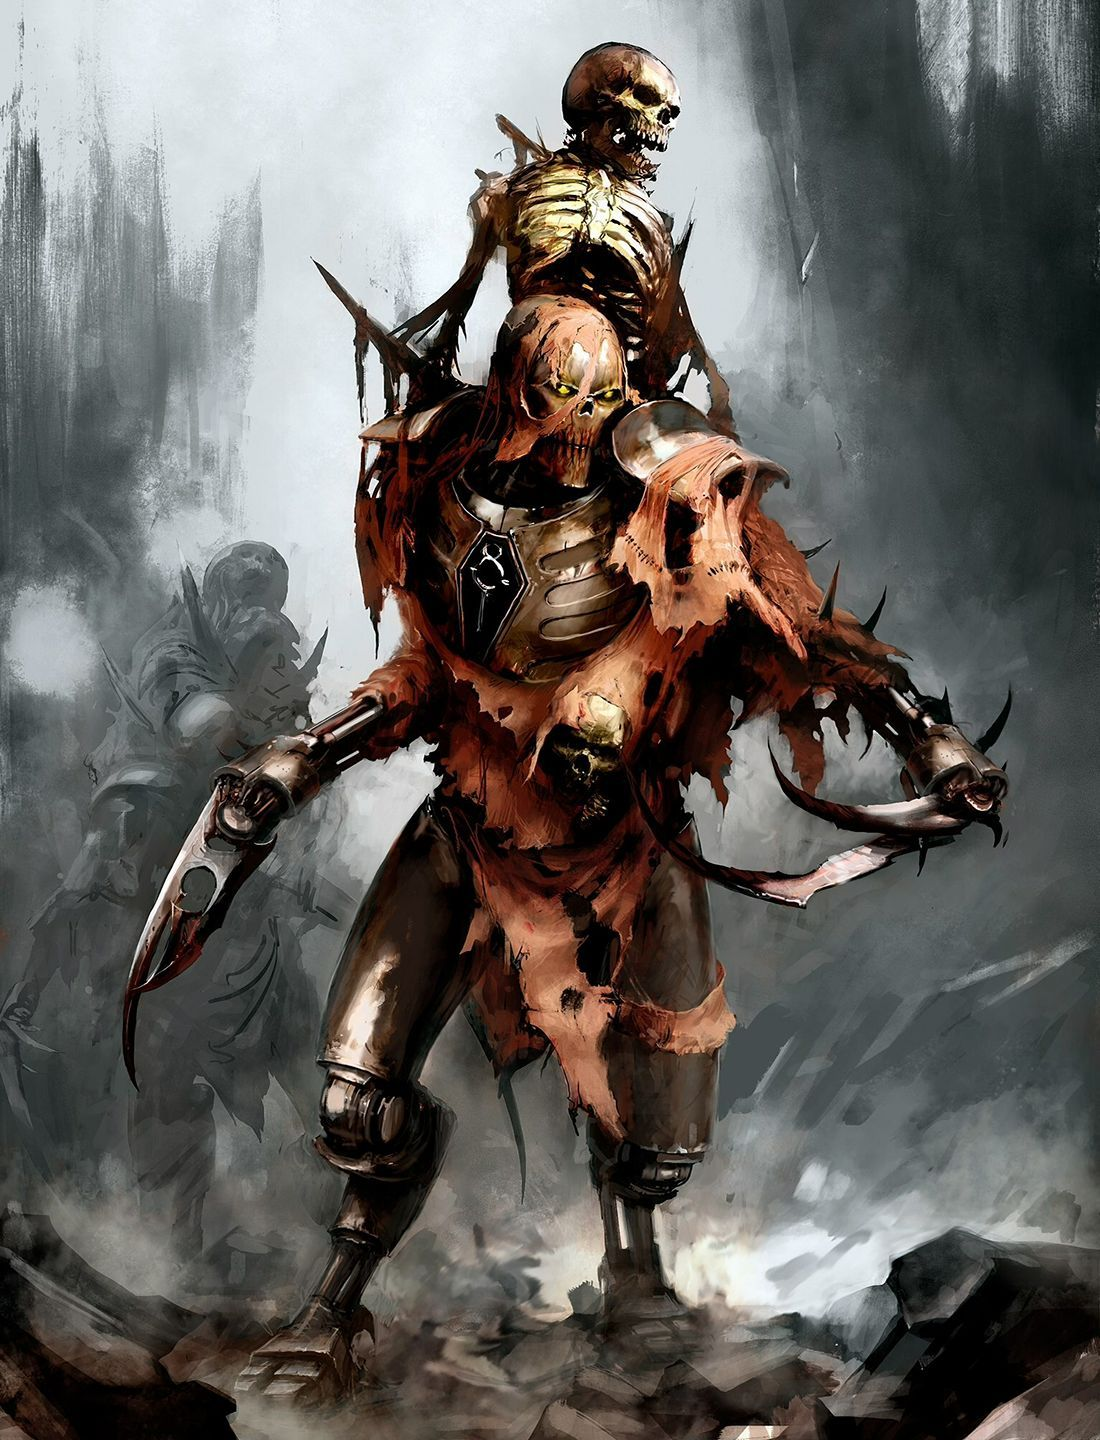
\includegraphics[height=530pt, width=400pt]{allied_art.jpg}
	\section[Allied Units]{\texorpdfstring{\centering\Huge Allied Units}{Allied Units}}
	
	\centerline{\begin{minipage}{400pt}
			\centering
			-
			
			\vspace*{1em}
			\raggedleft -
	\end{minipage}}
}

\newpage
\clearbackground

\label{allies}
\begin{tabular}{||c c c c c c c c c c c c c c c||}
	\hline
	\multicolumn{15}{||c||}{Primary Detachment} \\
	\multirow{14}{*}{\begin{sideways}Allied Detachment\end{sideways}} & & \begin{sideways}Charnovokh \end{sideways} & \begin{sideways}Maynarkh \end{sideways} & \begin{sideways}Mephrit \end{sideways} & \begin{sideways}Nephrekh \end{sideways} & \begin{sideways}Nihilakh \end{sideways} & \begin{sideways}Novokh \end{sideways} & \begin{sideways}Sautekh \end{sideways} & \begin{sideways}Szarekhan \end{sideways} & \begin{sideways}Thokt \end{sideways} & \begin{sideways}Triarch \end{sideways} & \begin{sideways}Destroyer Cult \end{sideways} & \begin{sideways}Flayed Ones \end{sideways} & \begin{sideways}Non-Necrons \end{sideways}\\
	& Charnovokh & & \greyskull & \blackskull & \blackskull & \blackskull & \blackskull & \blackskull & \redskull & \blackskull & \blackskull & \greyskull & \redskull & \redskull \\
	& Maynarhk & \greyskull & & \greyskull & \greyskull & \redskull & \blackskull & \greyskull & \blackskull & \greyskull & \blackskull & \blackskull & \blackskull & \redskull \\
	& Mephrit & \blackskull & \greyskull & & \greyskull & \greyskull  & \blackskull & \redskull & \yellowskull & \blackskull & \blackskull & \greyskull & \redskull & \redskull \\
	& Nephrekh & \blackskull & \greyskull & \greyskull & & \blackskull & \blackskull & \blackskull & \blackskull & \blackskull & \blackskull & \greyskull & \redskull & \redskull \\
	& Nihilakh & \blackskull & \redskull & \greyskull & \blackskull & & \greyskull & \blackskull & \yellowskull & \blackskull & \blackskull & \greyskull & \redskull & \redskull \\
	& Novokh & \blackskull & \blackskull & \blackskull & \blackskull & \greyskull & & \blackskull & \blackskull & \blackskull & \yellowskull & \yellowskull & \redskull & \redskull \\
	& Sautekh & \blackskull & \greyskull & \redskull & \blackskull & \blackskull & \blackskull & & \redskull & \greyskull & \greyskull & \greyskull & \redskull & \redskull \\
	& Szarekhan & \redskull & \blackskull & \yellowskull & \blackskull & \yellowskull & \blackskull & \redskull & & \yellowskull & \yellowskull & \greyskull & \redskull & \redskull \\
	& Thokt & \blackskull & \greyskull & \blackskull & \blackskull & \blackskull & \blackskull & \greyskull & \yellowskull & & \yellowskull & \greyskull & \redskull & \redskull \\
	& Triarch & \blackskull & \blackskull & \blackskull & \blackskull & \yellowskull & \blackskull & \greyskull & \yellowskull & \yellowskull & & \greyskull & \redskull & \redskull \\
	& Destroyer Cult & \greyskull & \blackskull & \greyskull & \greyskull & \greyskull & \yellowskull & \greyskull & \greyskull & \greyskull & \greyskull & & \greyskull & \redskull \\
	& Flayed Ones & \redskull & \blackskull & \redskull & \redskull & \redskull & \redskull & \redskull & \redskull & \redskull & \redskull & \greyskull & & \redskull \\
	& Non-Necrons & \redskull & \redskull & \redskull & \redskull & \redskull & \redskull & \redskull & \redskull & \redskull & \redskull & \redskull & \redskull & \\
	\hline
\end{tabular}

\subsection{Level of Alliance}

\noindent
\yellowskull Dynastic Allies

The closest of allies who have fought beside each other many times. The two forces are considered ‘friendly units’ in all regards. This means, for example, that Dynastic Allies may be joined by allied Independent Characters, are treated as friendly units for the targeting of special abilities, Warlord Traits and so on.

Note: Not even Dynastic Allies can embark in allied Transport Vehicles, and rules that affect a particular force owing to its Dynasty special rule do not carry over to Dynastic Allies allied units.

\noindent
\blackskull Fellow Warriors

The two forces are willing to fight together for common cause against their foes. Units in your army treat other units at the Fellow Warriors level of Alliance as not being part of the army with the exception that they may not be deliberately targeted, attacked, targeted with special abilities, etc, (note that Blasts and the like may still scatter over allied forces and adversely affect them).

Fellow Warriors cannot benefit from the effects of allied Warlord Traits or be joined by allied Independent Characters, and are not counted as friendly units for the purposes of special abilities. In essence, the two forces fight alongside each other without any additional positive or negative effect.

\noindent
\greyskull Distrusted Allies

The two forces can make common cause against an enemy, but never fully trust each other due to a long-standing feud or inherent antipathy. Models in the allied detachment are treated exactly like Fellow Warriors except that units in this allied detachment are never counted as Scoring units and may not hold Objectives.

\noindent
\redskull By the Phaeron's

The two forces will only ever fight beside each other in the direst of circumstances or by the direct command of their royal lord. The two forces are dealt with as Distrusted Allies but, in addition, whenever a unit is within 6" of a unit that is part of a Faction that falls under this level of alliance then both units reduce their Leadership by -1 until they are no longer within 6" of any unit from that Faction that is part of the same army.


\newpage
\subsection{Headquarters}

\newpage
\subsubsection[Destroyer Lord]{}

\fbox{\begin{imgminipage}{marble.jpg}[t]{0.2\textwidth}
		\color{white}
		\centering {\large (Destroyer Cult)\\HQ}
		
		\raggedright \small
		\color{black}
\end{imgminipage}}
\hspace{0.5em}
\begin{minipage}[t]{0.72\textwidth}
	{\large \textbf{Destroyer Lord \dotfill X points}}
	
	\begin{tabular}{m{160 pt} *{10}{c}}
		& M & WS & BS & S & T & W & I & A & Ld & Sv \\
		\hline
		Destroyer Lord & 9 & 4 & 4 & 5 & 6 & 4 & 2 & 4 & 10 & 3+ \\
	\end{tabular}
	\small
	\begin{minipage}[t]{0.5\textwidth}
		\begin{flushleft}
			\vspace*{2em}
			\textbf{Unit Composition}
			\begin{itemize}
				\item 1 Destroyer Lord
			\end{itemize}
			
			\textbf{Wargear}
			\begin{itemize}
				\item \quickref{Staff of Light}
			\end{itemize}
		\end{flushleft}
	\end{minipage}
	\begin{minipage}[t]{0.5\textwidth}
		\begin{flushleft}
			\vspace*{2em}
			\textbf{Unit Type}
			\begin{itemize}
				\item Infantry (Character, \quickref{Destroyer}, Floating, \quickref{Living Metal}, Noble)
			\end{itemize}
			
			\textbf{Special Rules}
			\begin{itemize}
				\item \quickref{Annihilation Protocols}
				\item Bulky (2)
				\item \quickref{Command Protocols}
				\item \quickref{Nodal Command} (Silver)
				\item \quickref{Reanimation Protocols}
				\item \quickref{Decurion Nemesor}
			\end{itemize}
		\end{flushleft}
	\end{minipage}
	
	\vspace*{2em}
	\textbf{Weapons}
	
	\begin{tabular}{L{90 pt} c C{40pt} *{2}{c} >{\raggedright\arraybackslash}p{130pt}}
		& Range & Type & S & AP & Abilities \\
		\hline
		\quickref{Staff of Light} & & &  &  &  \\
		— Shooting & 18" & Assault 3 & 5 & 3 & — \\
		— Melee & — & Melee & User & 3 & Rending (6+) \\
		\quickref{Hyperphase Sword} & — & Melee & User & 3 & Rending (5+) \\
		\quickref{Relic Gauss Blaster} & 30" & Rapid Fire & 5 & 4 & \quickref{Gauss} (6+), Twin-Linked \\	
		\quickref{Rod of Night} & & &  &  &  \\
		— Shooting & 18" & Assault 2 & 5 & — & Haywire, \quickref{Tesla} (6+) \\
		— Melee & — & Melee & User & — & \quickref{Energy Siphon}, Haywire \\
		\quickref{Voidblade} & — & Melee & User & 4 & \quickref{Entropic Strike} (4+), Rending(6+) \\
		\quickref{Warscythe} & — & Melee & +2 & 2 & Armourbane (Melee), Two-Handed \\
	\end{tabular}
	
	\vspace*{2em}
	\textbf{Options}
	\begin{itemize}
		\item The Destroyer Lord may exchange their \quickref{Staff of Light} for one of the following options:
		\begin{itemize}			
			\item \quickref{Hyperphase Sword} \dotfill -2 points
			\item \quickref{Rod of Night} \dotfill +5 points
			\item \quickref{Voidblade} \dotfill +0 points
			\item \quickref{Warscythe} \dotfill +20 points
			\item \quickref{Warscythe} with in-built \quickref{Relic Gauss Blaster} \dotfill +30 points
		\end{itemize}
		\item The Destroyer Lord may take any of the following options:
		\begin{itemize}
			\item \quickref{Gauntlet of Fire} \dotfill +10 points
			\item \quickref{Tachyon Arrow} \dotfill +50 points
			\item \quickref{Mindshackle Scarabs} \dotfill +20 points
			\item \quickref{Phase Shifter} \dotfill +25 points
			\item \quickref{Phylactery} \dotfill +10 points
			\item \quickref{Resurrection Orb} \dotfill +25 points
			\item \quickref{Sempiternal Weave} \dotfill +10 points
			\item \quickref{Tesseract Labyrinth} \dotfill +100 points
		\end{itemize}
		\item The Nemesor Lord may take equipment from the \quickref{Artefacts of the Aeons} list.
	\end{itemize}
\end{minipage}



\newpage
\subsubsection[Flayer King]{}

\begin{minipage}[t]{0.72\textwidth}
	{\large \textbf{Flayer King \dotfill X points}}
	
	\begin{tabular}{m{160 pt} *{10}{c}}
		& M & WS & BS & S & T & W & I & A & Ld & Sv \\
		\hline
		Flayer King & 7 & 5 & 4 & 5 & 5 & 4 & 2 & 3 & 10 & 3+ \\
	\end{tabular}
	\small
	\begin{minipage}[t]{0.5\textwidth}
		\begin{flushleft}
			\vspace*{2em}
			\textbf{Unit Composition}
			\begin{itemize}
				\item 1 Flayer King
			\end{itemize}
			
			\textbf{Wargear}
			\begin{itemize}
				\item \quickref{Staff of Light}
			\end{itemize}
		\end{flushleft}
	\end{minipage}
	\begin{minipage}[t]{0.5\textwidth}
		\begin{flushleft}
			\vspace*{2em}
			\textbf{Unit Type}
			\begin{itemize}
				\item Infantry (Character, \quickref{Flayer}, \quickref{Living Metal}, Noble)
			\end{itemize}
			
			\textbf{Special Rules}
			\begin{itemize}
				\item \quickref{Command Protocols}
				\item \quickref{Curse of Llandu'gor}
				\item \quickref{Drawn to Blood}
				\item \quickref{Hyperspace Hunters}
				\item \quickref{Mark of the Flayer}
				\item \quickref{Nodal Command} (Gold)
				\item \quickref{Reanimation Protocols}
				\item \quickref{Tesserarion Nemesor}
			\end{itemize}
		\end{flushleft}
	\end{minipage}
	
	\vspace*{2em}
	\textbf{Weapons}
	
	\begin{tabular}{L{90 pt} c C{40pt} *{2}{c} >{\raggedright\arraybackslash}p{130pt}}
		& Range & Type & S & AP & Abilities \\
		\hline
		\quickref{Staff of Light} & & &  &  &  \\
		— Shooting & 18" & Assault 3 & 5 & 3 & — \\
		— Melee & — & Melee & User & 3 & Rending (6+) \\
		\quickref{Hyperphase Sword} & — & Melee & User & 3 & Rending (5+) \\
		\quickref{Relic Gauss Blaster} & 30" & Rapid Fire & 5 & 4 & \quickref{Gauss} (6+), Twin-Linked \\	
		\quickref{Rod of Night} & & &  &  &  \\
		— Shooting & 18" & Assault 2 & 5 & — & Haywire, \quickref{Tesla} (6+) \\
		— Melee & — & Melee & User & — & \quickref{Energy Siphon}, Haywire \\
		\quickref{Voidblade} & — & Melee & User & 4 & \quickref{Entropic Strike} (4+), Rending(6+) \\
		\quickref{Voidscythe} & — & Melee & x2 & 1 & \quickref{Entropic Strike} (2+), Brutal (2), Unwieldy, Two-Handed \\
		\quickref{Warscythe} & — & Melee & +2 & 2 & Armourbane (Melee), Two-Handed \\
	\end{tabular}
	
	\vspace*{2em}
	\textbf{Options}
	\begin{itemize}
		\item The Flayer King may exchange their \quickref{Staff of Light} for one of the following options:
		\begin{itemize}			
			\item \quickref{Hyperphase Sword} \dotfill -2 points
			\item \quickref{Rod of Night} \dotfill +5 points
			\item \quickref{Voidblade} \dotfill +0 points
			\item \quickref{Warscythe} \dotfill +20 points
			\item \quickref{Warscythe} with in-built \quickref{Relic Gauss Blaster} \dotfill +30 points
		\end{itemize}
		\item The Flayer King may take any of the following options:
		\begin{itemize}
			\item \quickref{Gauntlet of Fire} \dotfill +10 points
			\item \quickref{Tachyon Arrow} \dotfill +150 points
			\item \quickref{Flensing Scarabs}\dotfill +10 points
			\item \quickref{Mindshackle Scarabs} \dotfill +20 points
			\item \quickref{Phase Shifter} \dotfill +25 points
			\item \quickref{Phylactery} \dotfill +10 points
			\item \quickref{Resurrection Orb} \dotfill +25 points
			\item \quickref{Sempiternal Weave} \dotfill +10 points
			\item \quickref{Shadow Ankh} \dotfill +10 points
			\item \quickref{Tesseract Labyrinth} \dotfill +100 points
			\item \quickref{Translocation Shroud} \dotfill +10 points
		\end{itemize}
		\item The Flayer King may take equipment from the \quickref{Artefacts of the Aeons} list.
	\end{itemize}
\end{minipage}
\hspace{0.5em}
\fbox{\begin{imgminipage}{marble.jpg}[t]{0.2\textwidth}
		\color{white}
		\centering {\large (Flayer Cult)\\HQ}
		
		\raggedright \small
		\color{black}
\end{imgminipage}}


\newpage
\subsubsection[Triarch High Judicator]{}

\fbox{\begin{imgminipage}{marble.jpg}[t]{0.2\textwidth}
		\color{white}
		\centering {\large (Triarch)\\HQ}
		
		\raggedright \small
		\color{black}
\end{imgminipage}}
\hspace{0.5em}
\begin{minipage}[t]{0.72\textwidth}
	{\large \textbf{High Judicator \dotfill X points}}
	
	\begin{tabular}{m{160 pt} *{10}{c}}
		& M & WS & BS & S & T & W & I & A & Ld & Sv \\
		\hline
		High Judicator & 7 & 5 & 5 & 5 & 5 & 4 & 2 & 3 & 10 & 3+ \\
	\end{tabular}
	\small
	\begin{minipage}[t]{0.5\textwidth}
		\begin{flushleft}
			\vspace*{2em}
			\textbf{Unit Composition}
			\begin{itemize}
				\item 1 High Judicator
			\end{itemize}
			
			\textbf{Wargear}
			\begin{itemize}
				\item \quickref{Rod of Covenant}
			\end{itemize}
		\end{flushleft}
	\end{minipage}
	\begin{minipage}[t]{0.5\textwidth}
		\begin{flushleft}
			\vspace*{2em}
			\textbf{Unit Type}
			\begin{itemize}
				\item Infantry (Character, \quickref{Living Metal}, \quickref{Noble})
			\end{itemize}
			
			\textbf{Special Rules}
			\begin{itemize}
				\item Bulky (2)
				\item \quickref{Command Protocols}
				\item Deep-Strike
				\item Fearless
				\item \quickref{Gravity Displacement Pack}
				\item Hammer of Wrath (1)
				\item My Will Be Done
				\item \quickref{Nodal Command} (Gold)
				\item \quickref{Reanimation Protocols}
				\item Relentless
				\item \quickref{Tesserarion Nemesor}
				\item Triarchial Duties
			\end{itemize}
		\end{flushleft}
	\end{minipage}
	
	\vspace*{2em}
	\textbf{Weapons}
	
	\begin{tabular}{L{90 pt} c C{40pt} *{2}{c} >{\raggedright\arraybackslash}p{130pt}}
		& Range & Type & S & AP & Abilities \\
		\hline
		\quickref{Rod of Covenant} &  &  &  &  & \\
		— Shooting & 12" & Assault 1 & 5 & 2 & — \\
		— Melee & — & Melee & User & 2 & Breaching (6+), Two-Handed \\
		\quickref{Particle Caster} & 12" & Pistol 1 & 6 & 5 & \\
		\quickref{Voidblade} & — & Melee & User & 4 & \quickref{Entropic Strike} (4+), Rending(6+) \\
		\quickref{Voidscythe} & — & Melee & x2 & 1 & \quickref{Entropic Strike} (2+), Brutal (2), Unwieldy, Two-Handed \\
	\end{tabular}
	
	\vspace*{2em}
	\textbf{Unit Rules}
	
	\textit{My Will Be Done:} A High Judicator automatically passes all Command Protocol checks.
	
	\textit{Triarchial Duties:} When selecting a High Judicator, an option from the Triarchial Duties options below must also be selected.
	
	\vspace*{2em}
	\textbf{Dedicated Transport}
	A High Judicator may take a Catacomb Command Barge as a Dedicated Transport. As a Dedicated Transport this does not use up an additional Force Organisation slot, but its points cost must still be paid for as part of the army.
	
	\vspace*{2em}
	\textbf{Options}
	\begin{itemize}
		\item The High Judicator must select one of the following Triarchial Duties options:
		\begin{itemize}
			\item Adjudicator: \dotfill +X points
			\item Executioner: +1 WS, BS, A \dotfill +X points
			\item Phaeron: \quickref{Nodal Command} (Platinum), Phaeron Sub-Type and Force Org slot \dotfill +X points
		\end{itemize}
		\item The High Judicator may exchange their \quickref{Rod of Covenant} for one of the following options:
		\begin{itemize}			
			\item \quickref{Voidscythe} \dotfill +X points
			\item \quickref{Voidblade} and \quickref{Particle Caster} \dotfill +X points
		\end{itemize}
		\item The High Judicator may take any of the following options:
		\begin{itemize}
			\item \quickref{Nyctotheric Optic Suite} \dotfill +15 points
			\item \quickref{Gauntlet of Fire} \dotfill +10 points
			\item \quickref{Tachyon Arrow} \dotfill +150 points
			\item \quickref{Mindshackle Scarabs} \dotfill +20 points
			\item \quickref{Phase Shifter} \dotfill +25 points
			\item \quickref{Phylactery} \dotfill +10 points
			\item \quickref{Resurrection Orb} \dotfill +25 points
			\item \quickref{Sempiternal Weave} \dotfill +10 points
			\item \quickref{Shadow Ankh} \dotfill +10 points
			\item \quickref{Tesseract Labyrinth} \dotfill +100 points
		\end{itemize}
		\item The High Judicator may take equipment from the \quickref{Artefacts of the Aeons} list.
	\end{itemize}
\end{minipage}


\newpage
\subsubsection[Skorpekh Lord]{}

\begin{minipage}[t]{0.72\textwidth}
	{\large \textbf{Skorpekh Lord \dotfill 163 points}}
	
	\begin{tabular}{m{160 pt} *{10}{c}}
		& M & WS & BS & S & T & W & I & A & Ld & Sv \\
		\hline
		Skorpekh Lord & 9 & 5 & 5 & 6 & 6 & 4 & 2 & 4 & 10 & 3+ \\
	\end{tabular}
	\small
	\begin{minipage}[t]{0.5\textwidth}
		\begin{flushleft}
			\vspace*{2em}
			\textbf{Unit Composition}
			\begin{itemize}
				\item 1 Skorpekh Lord
			\end{itemize}
			
			\textbf{Wargear}
			\begin{itemize}
				\item Close Combat Weapon
				\item \quickref{Enmitic Annihilator}
				\item \quickref{Hyperphase Harvester}
			\end{itemize}
		\end{flushleft}
	\end{minipage}
	\begin{minipage}[t]{0.5\textwidth}
		\begin{flushleft}
			\vspace*{2em}
			\textbf{Unit Type}
			\begin{itemize}
				\item Infantry (Character, \quickref{Destroyer}, \quickref{Living Metal}, Noble)
			\end{itemize}
			
			\textbf{Special Rules}
			\begin{itemize}
				\item \quickref{Annihilation Protocols}
				\item Bulky (3)
				\item \quickref{Command Protocols}
				\item Hammer of Wrath (1)
				\item \quickref{Nodal Command} (Gold)
				\item \quickref{Reanimation Protocols}
				\item Relentless
				\item \quickref{Tesserarion Nemesor}
			\end{itemize}
		\end{flushleft}
	\end{minipage}
	
	\vspace*{2em}
	\textbf{Weapons}
	
	\begin{tabular}{L{90 pt} c C{40pt} *{2}{c} >{\raggedright\arraybackslash}p{130pt}}
		& Range & Type & S & AP & Abilities \\
		\hline
		\quickref{Enmitic Annihilator} & 18" & Assault 1 & 6 & 4 & Blast, Molecular Dissonance \\
		\quickref{Hyperphase Harvester} & — & Melee & +2 & 2 & Murderous Strike (4+), Two-Handed, Unwieldy \\
	\end{tabular}
	
	\vspace*{2em}
	\textbf{Options}
	\begin{itemize}
		\item The Skorpekh Lord may take any of the following options:
		\begin{itemize}
			\item \quickref{Mindshackle Scarabs} \dotfill +20 points
			\item \quickref{Phase Shifter} \dotfill +25 points
			\item \quickref{Phylactery} \dotfill +10 points
			\item \quickref{Sempiternal Weave} \dotfill +10 points
			\item \quickref{Shadow Ankh} \dotfill +10 points
			\item \quickref{Tesseract Labyrinth} \dotfill +100 points
		\end{itemize}
		\item The Skorpekh Lord may take equipment from the \quickref{Artefacts of the Aeons} list.
	\end{itemize}
\end{minipage}
\hspace{0.5em}
\fbox{\begin{imgminipage}{marble.jpg}[t]{0.2\textwidth}
		\color{white}
		\centering {\large (Destroyer Cult)\\HQ}
		
		\raggedright \small
		\color{black}
\end{imgminipage}}


\newpage
\subsection{Elites}

\newpage
\subsubsection[Charnel Lychguard Phalanx]{}
\begin{minipage}[t]{0.72\textwidth}
	{\large \textbf{Charnel Lychguard Phalanx \dotfill X Points}}
	
	\begin{tabular}{m{160 pt} *{10}{c}}
		& M & WS & BS & S & T & W & I & A & Ld & Sv \\
		\hline
		Charnel Lychguard & 7 & 4 & 4 & 5 & 5 & 1 & 2 & 2 & 10 & 3+ \\
	\end{tabular}
	\small
	\begin{minipage}[t]{0.5\textwidth}
		\begin{flushleft}
			\vspace*{2em}
			\textbf{Unit Composition}
			\begin{itemize}
				\item 5 Charnel Lychguard
			\end{itemize}
			
			\textbf{Wargear}
			\begin{itemize}
				\item \quickref{Warscythe}
			\end{itemize}
		\end{flushleft}
	\end{minipage}
	\begin{minipage}[t]{0.5\textwidth}
		\begin{flushleft}
			\vspace*{2em}
			\textbf{Unit Type}
			\begin{itemize}
				\item Infantry (Flayer, Line, \quickref{Living Metal})
			\end{itemize}
			
			\textbf{Special Rules}
			\begin{itemize}
				\item \quickref{Awakening Protocols} (Bronze)
				\item Chosen Warriors
				\item \quickref{Curse of Llandu'gor}
				\item Rage (1)
				\item \quickref{Reanimation Protocols}
				\item Soldier of the Bloody Court
			\end{itemize}
		\end{flushleft}
	\end{minipage}
	
	\vspace*{2em}
	\textbf{Weapons}
	
	\begin{tabular}{L{90 pt} c C{40pt} *{2}{c} >{\raggedright\arraybackslash}p{130pt}}
		& Range & Type & S & AP & Abilities \\
		\hline
		\quickref{Hyperphase Sword} & — & Melee & User & 3 & Rending (5+) \\
		\quickref{Warscythe} & — & Melee & +2 & 2 & Armourbane (Melee), Two-Handed \\
		\quickref{Gauss Blaster} & 24" & Rapid Fire 1 & 5 & 4 & \quickref{Gauss} (6+) \\
	\end{tabular}
	
	\vspace*{2em}
	\textbf{Unit Rules}
	
	\textit{Soldier of the Bloody Court:} Only a single Royal or Charnel Lychguard Phalanx unit may be purchased for each Lord, Nemesor Lord, Nemesor Overlord, and/or Phaeron and are treated as their personal retinue. This does not use up an additional Force Organisation slot and they do not have to be deployed with them. They count as within Nodal Command Range of their respective HQ while they are both on the table.
		
	\vspace*{2em}
	\textbf{Dedicated Transport}
	A Charnel Lychguard Phalanx may take a Night Scythe as a Dedicated Transport. As a Dedicated Transport this does not use up an additional Force Organisation slot, but its points cost must still be paid for as part of the army.
	
	\vspace*{2em}
	\textbf{Options}
	\begin{itemize}
		\item The Charnel Lychguard Phalanx may include:
		\begin{itemize}
			\item Up to an additional 5 Charnel Lychguards \dotfill X points each
		\end{itemize}
		\item The entire unit may exchange their \quickref{Warscythe} for one of the following options:
		\begin{itemize}
			\item \quickref{Warscythe} with in-built \quickref{Gauss Blaster} \dotfill +5 points each
			\item \quickref{Hyperphase Sword} and \quickref{Dispension Shield} \dotfill +10 points each
		\end{itemize}
		\item The entire unit may take the following option:
		\begin{itemize}
			\item \quickref{Flensing Scarabs} \dotfill +10 points each
		\end{itemize}
	\end{itemize}
\end{minipage}
\hspace{0.5em}
\fbox{\begin{imgminipage}{marble.jpg}[t]{0.2\textwidth}
		\color{white}
		\centering {\large (Flayer Cult)\\ELITES}
		
		\raggedright \small
		\color{black}
\end{imgminipage}}


\newpage
\subsubsection[Flayed Ones Pack]{}
\begin{minipage}[t]{0.72\textwidth}
	{\large \textbf{Flayed Ones Pack \dotfill X Points}}
	
	\begin{tabular}{m{160 pt} *{10}{c}}
		& M & WS & BS & S & T & W & I & A & Ld & Sv \\
		\hline
		Flayed One & 6 & 4 & 1 & 4 & 4 & 1 & 2 & 3 & 10 & 4+ \\
	\end{tabular}
	\small
	\begin{minipage}[t]{0.5\textwidth}
		\begin{flushleft}
			\vspace*{2em}
			\textbf{Unit Composition}
			\begin{itemize}
				\item 5 Flayed Ones
			\end{itemize}
			
			\textbf{Wargear}
			\begin{itemize}
				\item Two Close Combat Weapons
			\end{itemize}
		\end{flushleft}
	\end{minipage}
	\begin{minipage}[t]{0.5\textwidth}
		\begin{flushleft}
			\vspace*{2em}
			\textbf{Unit Type}
			\begin{itemize}
				\item Infantry (Flayer, \quickref{Living Metal})
			\end{itemize}
			
			\textbf{Special Rules}
			\begin{itemize}
				\item \quickref{Curse of Llandu'gor}
				\item \quickref{Drawn to Blood}
				\item \quickref{Hyperspace Hunters}
				\item \quickref{Reanimation Protocols}
			\end{itemize}
		\end{flushleft}
	\end{minipage}
		
	\vspace*{2em}
	\textbf{Options}
	\begin{itemize}
		\item The Flayed Ones Pack may include:
		\begin{itemize}
			\item Up to an additional 15 Flayed Ones \dotfill X points each
		\end{itemize}
		\item The entire unit may take the following option:
		\begin{itemize}
			\item \quickref{Flensing Scarabs} \dotfill +10 points each
		\end{itemize}
	\end{itemize}
\end{minipage}
\hspace{0.5em}
\fbox{\begin{imgminipage}{marble.jpg}[t]{0.2\textwidth}
		\color{white}
		\centering {\large (Flayer Cult)\\ELITES}
		
		\raggedright \small
		\color{black}
\end{imgminipage}}



\newpage
\subsubsection[Hexmark Destroyer]{}
\begin{minipage}[t]{0.72\textwidth}
	{\large \textbf{Hexmark Destroyer \dotfill X Points}}
	
	\begin{tabular}{m{160 pt} *{10}{c}}
		& M & WS & BS & S & T & W & I & A & Ld & Sv \\
		\hline
		Hexmark Destroyer & 9 & 4 & 6 & 5 & 5 & 3 & 2 & 3 & 10 & 3+ \\
	\end{tabular}
	\small
	\begin{minipage}[t]{0.5\textwidth}
		\begin{flushleft}
			\vspace*{2em}
			\textbf{Unit Composition}
			\begin{itemize}
				\item 1 Hexmark Destroyer
			\end{itemize}
			
			\textbf{Wargear}
			\begin{itemize}
				\item Six \quickref{Enmitic Disintegrator Pistol}s
			\end{itemize}
		\end{flushleft}
	\end{minipage}
	\begin{minipage}[t]{0.5\textwidth}
		\begin{flushleft}
			\vspace*{2em}
			\textbf{Unit Type}
			\begin{itemize}
				\item Infantry (Character, Destroyer, \quickref{Living Metal})
			\end{itemize}
			
			\textbf{Special Rules}
			\begin{itemize}
				\item \quickref{Annihilation Protocols}
				\item \quickref{Awakening Protocols} (Silver)
				\item Bulky (3)
				\item Deep-Strike
				\item \quickref{Ethereal Interceptors}
				\item Firing Protocols (6)
				\item Inescapable Death
				\item Multi-Threat Eliminator
				\item \quickref{Reanimation Protocols}
				\item \quickref{Hyperspace Hunters}
			\end{itemize}
		\end{flushleft}
	\end{minipage}
	
	\vspace*{2em}
	\textbf{Weapons}
	
	\begin{tabular}{L{90 pt} c C{40pt} *{2}{c} >{\raggedright\arraybackslash}p{130pt}}
		& Range & Type & S & AP & Abilities \\
		\hline
		\quickref{Enmitic Disintegrator Pistol} & 18" & Pistol 1 & 6 & 4 & Molecular Dissonance \\
	\end{tabular}
	
	\vspace*{2em}
	\textbf{Unit Rules}
		
	\textit{Inescapable Death:} The Hexmark Destroyer has full BS when firing Snap Shots. In addition all of its Weapons gain the Precision Shot (4+) and Ignores cover special rules and it cannot have its BS reduced.
	
	\textit{Multi-Threat Eliminator:} This model may target different units with each of its weapons. In addition, each time an enemy model is destroyed by a ranged attack made by this model's enmitic disintegrator pistols, after this model makes the rest of its attacks, it can shoot with one of its enmitic disintegrator pistols one additional time. These attacks cannot generate additional attacks.
		
	\vspace*{2em}
	\textbf{Options}
	\begin{itemize}
		\item The Hexmark Destroyer may take any of the following options:
		\begin{itemize}
			\item \quickref{Hyper-Oubliette Navigator} \dotfill +5 points each
		\end{itemize}
	\end{itemize}
\end{minipage}
\hspace{0.5em}
\fbox{\begin{imgminipage}{marble.jpg}[t]{0.2\textwidth}
		\color{white}
		\centering {\large (Destroyer Cult)\\ELITES}
		
		\raggedright \small
		\color{black}
\end{imgminipage}}


\newpage
\subsubsection[Skorpekh Destroyer Vanguard]{}

\begin{minipage}[t]{0.72\textwidth}
	{\large \textbf{Skorpekh Destroyer Vanguard \dotfill 114 points}}
	
	\begin{tabular}{m{160 pt} *{10}{c}}
		& M & WS & BS & S & T & W & I & A & Ld & Sv \\
		\hline
		Skorpekh Destroyer & 9 & 4 & 4 & 5 & 5 & 3 & 2 & 3 & 10 & 3+ \\
	\end{tabular}
	\small
	\begin{minipage}[t]{0.5\textwidth}
		\begin{flushleft}
			\vspace*{2em}
			\textbf{Unit Composition}
			\begin{itemize}
				\item 3 Skorpekh Destroyers
			\end{itemize}
			
			\textbf{Wargear}
			\begin{itemize}
				\item Two \quickref{Hyperphase Thresher}s
			\end{itemize}
		\end{flushleft}
	\end{minipage}
	\begin{minipage}[t]{0.5\textwidth}
		\begin{flushleft}
			\vspace*{2em}
			\textbf{Unit Type}
			\begin{itemize}
				\item Infantry (\quickref{Destroyer}, \quickref{Living Metal})
			\end{itemize}
			
			\textbf{Special Rules}
			\begin{itemize}
				\item \quickref{Annihilation Protocols}
				\item \quickref{Awakening Protocols} (Silver)
				\item Bulky (3)
				\item Hammer of Wrath (1)
				\item \quickref{Reanimation Protocols}
			\end{itemize}
		\end{flushleft}
	\end{minipage}
	
	\vspace*{2em}
	\textbf{Weapons}
	
	\begin{tabular}{L{90 pt} c C{40pt} *{2}{c} >{\raggedright\arraybackslash}p{130pt}}
		& Range & Type & S & AP & Abilities \\
		\hline
		\quickref{Hyperphase Reap-Blade} & — & Melee & +2 & 2 & Murderous Strike (5+), Two-Handed \\
		\quickref{Hyperphase Thresher} & — & Melee & User & 3 & Reaping Blow (1), Specialist Weapon \\
	\end{tabular}
	
	\vspace*{2em}
	\textbf{Options}
	\begin{itemize}
		\item The Skorpekh Destroyer Vanguard may include:
		\begin{itemize}
			\item Up to an additional 3 Skorpekh Destroyers \dotfill +38 points each
		\end{itemize}
		\item Any model may exchange two \quickref{Hyperphase Thresher}s for a:
		\begin{itemize}
			\item \quickref{Hyperphase Reap-Blade} \dotfill +15 points
		\end{itemize}
	\end{itemize}
\end{minipage}
\hspace{0.5em}
\fbox{\begin{imgminipage}{marble.jpg}[t]{0.2\textwidth}
		\color{white}
		\centering {\large (Destroyer Cult)\\ELITES}
		
		\raggedright \small
		\color{black}
\end{imgminipage}}




\newpage
\subsubsection[Triarch Judicator Vanguard]{}

\begin{minipage}[t]{0.72\textwidth}
	{\large \textbf{Triarch Judicator Vanguard \dotfill X points}}
	
	\begin{tabular}{m{160 pt} *{10}{c}}
		& M & WS & BS & S & T & W & I & A & Ld & Sv \\
		\hline
		Triarch Judicator & 7 & 5 & 5 & 5 & 5 & 2 & 2 & 3 & 10 & 3+ \\
	\end{tabular}
	\small
	\begin{minipage}[t]{0.5\textwidth}
		\begin{flushleft}
			\vspace*{2em}
			\textbf{Unit Composition}
			\begin{itemize}
				\item 3 Triarch Judicators
			\end{itemize}
			
			\textbf{Wargear}
			\begin{itemize}
				\item \quickref{Rod of Covenant}
			\end{itemize}
		\end{flushleft}
	\end{minipage}
	\begin{minipage}[t]{0.5\textwidth}
		\begin{flushleft}
			\vspace*{2em}
			\textbf{Unit Type}
			\begin{itemize}
				\item Infantry (\quickref{Living Metal})
			\end{itemize}
			
			\textbf{Special Rules}
			\begin{itemize}
				\item Bulky (2)
				\item Deep-Strike
				\item Fearless
				\item \quickref{Gravity Displacement Pack}
				\item Hammer of Wrath (1)
				\item \quickref{Reanimation Protocols}
			\end{itemize}
		\end{flushleft}
	\end{minipage}
	
	\vspace*{2em}
	\textbf{Weapons}
	
	\begin{tabular}{L{90 pt} c C{40pt} *{2}{c} >{\raggedright\arraybackslash}p{130pt}}
		& Range & Type & S & AP & Abilities \\
		\hline
		\quickref{Rod of Covenant} &  &  &  &  & \\
		— Shooting & 12" & Assault 1 & 5 & 2 & — \\
		— Melee & — & Melee & User & 2 & Breaching (6+), Two-Handed \\
		\quickref{Particle Caster} & 12" & Pistol 1 & 6 & 5 & \\
		\quickref{Voidblade} & — & Melee & User & 4 & \quickref{Entropic Strike} (4+), Rending(6+) \\
	\end{tabular}
	
	\vspace*{2em}
	\textbf{Dedicated Transport}
	A Triarch Praetorian Vanguard may take a Night Scythe as a Dedicated Transport. As a Dedicated Transport this does not use up an additional Force Organisation slot, but its points cost must still be paid for as part of the army.
	
	\vspace*{2em}
	\textbf{Options}
	\begin{itemize}
		\item The Triarch Judicator Vanguard may include:
		\begin{itemize}
			\item Up to an additional 7 Triarch Judicator \dotfill +X points each
		\end{itemize}
		\item Each model may exchange its \quickref{Rod of Covenant} for:
		\begin{itemize}
			\item \quickref{Voidblade} and \quickref{Particle Caster} \dotfill +X points each
		\end{itemize}
		\item Each model may take any of the following options:
		\begin{itemize}
			\item \quickref{Phase Shifter} \dotfill +25 points each
			\item \quickref{Phylactery} \dotfill +10 points each
			\item \quickref{Sempiternal Weave} \dotfill +10 points each
		\end{itemize}
	\end{itemize}
\end{minipage}
\hspace{0.5em}
\fbox{\begin{imgminipage}{marble.jpg}[t]{0.2\textwidth}
		\color{white}
		\centering {\large (Triarch)\\FAST ATTACK}
		
		\raggedright \small
		\color{black}
\end{imgminipage}}


\newpage
\subsection{Fast Attack}

\newpage
\subsubsection[Charnel Scarab Swarms]{}

\fbox{\begin{imgminipage}{marble.jpg}[t]{0.2\textwidth}
		\color{white}
		\centering {\large (Flayer Cult)\\FAST ATTACK}
		
		\raggedright \small
		\color{black}
\end{imgminipage}}
\hspace{0.5em}
\begin{minipage}[t]{0.72\textwidth}
	{\large \textbf{Charnel Scarab Swarms \dotfill X Points}}
	
	\begin{tabular}{m{160 pt} *{10}{c}}
		& M & WS & BS & S & T & W & I & A & Ld & Sv \\
		\hline
		Charnel Scarab Swarm & 10 & 3 & 2 & 3 & 3 & 3 & 2 & 4 & 10 & 6+ \\
	\end{tabular}
	\small
	\begin{minipage}[t]{0.5\textwidth}
		\begin{flushleft}
			\vspace*{2em}
			\textbf{Unit Composition}
			\begin{itemize}
				\item 3 Charnel Scarab Swarms
			\end{itemize}
			
			\textbf{Wargear}
			\begin{itemize}
				\item Charnel Maws
			\end{itemize}
		\end{flushleft}
	\end{minipage}
	\begin{minipage}[t]{0.5\textwidth}
		\begin{flushleft}
			\vspace*{2em}
			\textbf{Unit Type}
			\begin{itemize}
				\item Infantry (Canoptek, Floating, Light, \quickref{Living Metal}, Monstrous)
			\end{itemize}
			
			\textbf{Special Rules}
			\begin{itemize}
				\item \quickref{Reanimation Protocols}
				\item \quickref{Soulless Hordes} (Bronze)
				\item Swarms
			\end{itemize}
		\end{flushleft}
	\end{minipage}
	
	\vspace*{2em}
	\textbf{Weapons}
	
	\begin{tabular}{L{90 pt} c C{40pt} *{2}{c} >{\raggedright\arraybackslash}p{130pt}}
		& Range & Type & S & AP & Abilities \\
		Charnel Maws & — & Melee & User & — & Shred, Rending (6+) \\
	\end{tabular}
		
	\vspace*{2em}
	\textbf{Options}
	\begin{itemize}
		\item The Charnel Scarab Swarms may include:
		\begin{itemize}
			\item Up to an additional 6 Charnel Scarab Swarm models \dotfill X points each
		\end{itemize}
	\end{itemize}
\end{minipage}


\newpage
\subsubsection[Triarch Praetorian Vanguard]{}

\begin{minipage}[t]{0.72\textwidth}
	{\large \textbf{Triarch Praetorian Vanguard \dotfill X points}}
	
	\begin{tabular}{m{160 pt} *{10}{c}}
		& M & WS & BS & S & T & W & I & A & Ld & Sv \\
		\hline
		Triarch Praetorian & 7 & 4 & 4 & 5 & 5 & 1 & 2 & 2 & 10 & 3+ \\
		Triarch Judicator & 7 & 5 & 5 & 5 & 5 & 2 & 2 & 3 & 10 & 3+ \\
	\end{tabular}
	\small
	\begin{minipage}[t]{0.5\textwidth}
		\begin{flushleft}
			\vspace*{2em}
			\textbf{Unit Composition}
			\begin{itemize}
				\item 3 Triarch Praetorians
			\end{itemize}
			
			\textbf{Wargear}
			\begin{itemize}
				\item \quickref{Rod of Covenant}
			\end{itemize}
		\end{flushleft}
	\end{minipage}
	\begin{minipage}[t]{0.5\textwidth}
		\begin{flushleft}
			\vspace*{2em}
			\textbf{Unit Type}
			\begin{itemize}
				\item Infantry (\quickref{Living Metal})
			\end{itemize}
			
			\textbf{Special Rules}
			\begin{itemize}
				\item Bulky (2)
				\item Deep-Strike
				\item Fearless
				\item \quickref{Gravity Displacement Pack}
				\item Hammer of Wrath (1)
				\item \quickref{Reanimation Protocols}
			\end{itemize}
		\end{flushleft}
	\end{minipage}
	
	\vspace*{2em}
	\textbf{Weapons}
	
	\begin{tabular}{L{90 pt} c C{40pt} *{2}{c} >{\raggedright\arraybackslash}p{130pt}}
		& Range & Type & S & AP & Abilities \\
		\hline
		\quickref{Rod of Covenant} &  &  &  &  & \\
		— Shooting & 12" & Assault 1 & 5 & 2 & — \\
		— Melee & — & Melee & User & 2 & Breaching (6+), Two-Handed \\
		\quickref{Particle Caster} & 12" & Pistol 1 & 6 & 5 & \\
		\quickref{Voidblade} & — & Melee & User & 4 & \quickref{Entropic Strike} (4+), Rending(6+) \\
	\end{tabular}
	
	\vspace*{2em}
	\textbf{Dedicated Transport}
	A Triarch Praetorian Vanguard may take a Night Scythe as a Dedicated Transport. As a Dedicated Transport this does not use up an additional Force Organisation slot, but its points cost must still be paid for as part of the army.
	
	\vspace*{2em}
	\textbf{Options}
	\begin{itemize}
		\item The Triarch Praetorian Vanguard may include:
		\begin{itemize}
			\item Up to an additional 7 Triarch Praetorians \dotfill +X points each
		\end{itemize}
		\item Up to one Triarch Praetorian may be upgraded to a:
		\begin{itemize}
			\item Triarch Judicator \dotfill +X points each
		\end{itemize}
		\item Each model may exchange its \quickref{Rod of Covenant} for:
		\begin{itemize}
			\item \quickref{Voidblade} and \quickref{Particle Caster} \dotfill +X points each
		\end{itemize}
		\item Each model may take any of the following options:
		\begin{itemize}
			\item \quickref{Phase Shifter} \dotfill +25 points each
			\item \quickref{Phylactery} \dotfill +10 points each
			\item \quickref{Sempiternal Weave} \dotfill +10 points each
		\end{itemize}
	\end{itemize}
\end{minipage}
\hspace{0.5em}
\fbox{\begin{imgminipage}{marble.jpg}[t]{0.2\textwidth}
		\color{white}
		\centering {\large (Triarch)\\FAST ATTACK}
		
		\raggedright \small
		\color{black}
\end{imgminipage}}

\newpage
\subsubsection[Ophydian Destroyer Vanguard]{}

\fbox{\begin{imgminipage}{marble.jpg}[t]{0.2\textwidth}
		\color{white}
		\centering {\large (Destroyer Cult)\\FAST ATTACK}
		
		\raggedright \small
		\color{black}
\end{imgminipage}}
\hspace{0.5em}
\begin{minipage}[t]{0.72\textwidth}
	{\large \textbf{Ophydian Destroyer Vanguard \dotfill X points}}
	
	\begin{tabular}{m{160 pt} *{10}{c}}
		& M & WS & BS & S & T & W & I & A & Ld & Sv \\
		\hline
		Ophydian Destroyer & 10 & 4 & 4 & 4 & 4 & 2 & 2 & 3 & 10 & 4+ \\
	\end{tabular}
	\small
	\begin{minipage}[t]{0.5\textwidth}
		\begin{flushleft}
			\vspace*{2em}
			\textbf{Unit Composition}
			\begin{itemize}
				\item 3 Ophydian Destroyers
			\end{itemize}
			
			\textbf{Wargear}
			\begin{itemize}
				\item Two \quickref{Hyperphase Thresher}s
				\item \quickref{Whip Coils}
			\end{itemize}
		\end{flushleft}
	\end{minipage}
	\begin{minipage}[t]{0.5\textwidth}
		\begin{flushleft}
			\vspace*{2em}
			\textbf{Unit Type}
			\begin{itemize}
				\item Infantry (\quickref{Destroyer}, \quickref{Living Metal})
			\end{itemize}
			
			\textbf{Special Rules}
			\begin{itemize}
				\item \quickref{Annihilation Protocols}
				\item \quickref{Awakening Protocols} (Silver)
				\item Bulky (3)
				\item Hammer of Wrath (2)
				\item \quickref{Reanimation Protocols}
				\item Subterranean Assault
			\end{itemize}
		\end{flushleft}
	\end{minipage}
	
	\vspace*{2em}
	\textbf{Weapons}
	
	\begin{tabular}{L{90 pt} c C{40pt} *{2}{c} >{\raggedright\arraybackslash}p{130pt}}
		& Range & Type & S & AP & Abilities \\
		\hline
		\quickref{Hyperphase Reap-Blade} & — & Melee & +2 & 2 & Murderous Strike (5+), Two-Handed \\
		\quickref{Hyperphase Thresher} & — & Melee & User & 3 & Reaping Blow (1), Specialist Weapon \\
		\quickref{Whip Coils} & — & Melee & User & — & Reach (3) \\
	\end{tabular}
	
	\vspace*{2em}
	\textbf{Options}
	\begin{itemize}
		\item The Ophydian Destroyer Vanguard may include:
		\begin{itemize}
			\item Up to an additional 3 Ophydian Destroyers \dotfill X points each
		\end{itemize}
		\item Each model may exchange two \quickref{Hyperphase Thresher}s for a:
		\begin{itemize}
			\item \quickref{Hyperphase Reap-Blade} \dotfill +X points
		\end{itemize}
	\end{itemize}
\end{minipage}



\newpage
\subsection{Heavy Support}

\newpage
\subsubsection[Lokhust Destroyer Clave]{}

\begin{minipage}[t]{0.72\textwidth}
	{\large \textbf{Lokhust Destroyer Clave \dotfill X points}}
	
	\begin{tabular}{m{160 pt} *{10}{c}}
		& M & WS & BS & S & T & W & I & A & Ld & Sv \\
		\hline
		Lokhust Destroyer & 9 & 4 & 4 & 4 & 5 & 2 & 2 & 3 & 10 & 3+ \\
		Lokhust Heavy Destroyer & 9 & 4 & 4 & 4 & 5 & 3 & 2 & 3 & 10 & 3+ \\
	\end{tabular}
	\small
	\begin{minipage}[t]{0.5\textwidth}
		\begin{flushleft}
			\vspace*{2em}
			\textbf{Unit Composition}
			\begin{itemize}
				\item 1 Lokhust Destroyer
			\end{itemize}
			
			\textbf{Wargear}
			\begin{itemize}
				\item \quickref{Gauss Cannon}
			\end{itemize}
		\end{flushleft}
	\end{minipage}
	\begin{minipage}[t]{0.5\textwidth}
		\begin{flushleft}
			\vspace*{2em}
			\textbf{Unit Type}
			\begin{itemize}
				\item Infantry (\quickref{Destroyer}, Floating, \quickref{Living Metal})
			\end{itemize}
			
			\textbf{Special Rules}
			\begin{itemize}
				\item \quickref{Annihilation Protocols}
				\item \quickref{Awakening Protocols} (Bronze)
				\item Bulky (2)
				\item \quickref{Reanimation Protocols}
				\item Relentless
			\end{itemize}
		\end{flushleft}
	\end{minipage}
	
	\vspace*{2em}
	\textbf{Weapons}
	
	\begin{tabular}{L{90 pt} c C{40pt} *{2}{c} >{\raggedright\arraybackslash}p{130pt}}
		& Range & Type & S & AP & Abilities \\
		\hline
		\quickref{Enmitic Exterminator} & 36" & Heavy 1 & 7 & 4 & Large Blast, Molecular Dissonance \\
		\quickref{Gauss Cannon} & 24" & Heavy 3 & 6 & 2 & \quickref{Gauss} (6+) \\
		\quickref{Gauss Destructor} & 36" & Heavy 1 & 10 & 1 &  \quickref{Gauss} (6+) \\
		\quickref{Tesla Cannon} & 24" & Heavy 2 & 6 & — & \quickref{Tesla} (6+) \\
		\quickref{Tesla Destructor} & 36" & Heavy 4 & 7 & — &  \quickref{Tesla} (6+) \\
	\end{tabular}
	
	\vspace*{2em}
	\textbf{Options}
	\begin{itemize}
		\item The Lokhust Destroyer Clade may include:
		\begin{itemize}
			\item Up to an additional 5 Lokhust Destroyers \dotfill X points each
		\end{itemize}
		\item Up to one Lokhust Destroyer may be upgraded to a:
		\begin{itemize}
			\item Lokhust Heavy Destroyer equipped with a \quickref{Gauss Destructor} \dotfill X points
		\end{itemize}
		\item Each Lokhust Destroyer may exchange its \quickref{Gauss Cannon} one of the following options:
		\begin{itemize}
			\item \quickref{Tesla Cannon} \dotfill +X points
		\end{itemize}
		\item Each Lokhust Heavy Destroyer may exchange its \quickref{Gauss Destructor} one of the following options:
		\begin{itemize}
			\item \quickref{Enmitic Exterminator} \dotfill +X points
			\item \quickref{Tesla Destructor} \dotfill +X points
		\end{itemize}
	\end{itemize}
\end{minipage}
\hspace{0.5em}
\fbox{\begin{imgminipage}{marble.jpg}[t]{0.2\textwidth}
		\color{white}
		\centering {\large (Destroyer Cult)\\HEAVY SUPPORT}
		
		\raggedright \small
		\color{black}
\end{imgminipage}}


\newpage
\subsubsection[Lokhust Heavy Destroyer Clave]{}

\begin{minipage}[t]{0.72\textwidth}
	{\large \textbf{Lokhust Heavy Destroyer Clave \dotfill 45 points}}
	
	\begin{tabular}{m{160 pt} *{10}{c}}
		& M & WS & BS & S & T & W & I & A & Ld & Sv \\
		\hline
		Lokhust Heavy Destroyer & 9 & 4 & 4 & 4 & 5 & 3 & 2 & 2 & 10 & 3+ \\
	\end{tabular}
	\small
	\begin{minipage}[t]{0.5\textwidth}
		\begin{flushleft}
			\vspace*{2em}
			\textbf{Unit Composition}
			\begin{itemize}
				\item 1 Lokhust Heavy Destroyer
			\end{itemize}
			
			\textbf{Wargear}
			\begin{itemize}
				\item \quickref{Gauss Destructor}
			\end{itemize}
		\end{flushleft}
	\end{minipage}
	\begin{minipage}[t]{0.5\textwidth}
		\begin{flushleft}
			\vspace*{2em}
			\textbf{Unit Type}
			\begin{itemize}
				\item Infantry (\quickref{Destroyer}, Floating, \quickref{Living Metal})
			\end{itemize}
			
			\textbf{Special Rules}
			\begin{itemize}
				\item \quickref{Annihilation Protocols}
				\item \quickref{Awakening Protocols} (Silver)
				\item Bulky (2)
				\item \quickref{Reanimation Protocols}
				\item Relentless
			\end{itemize}
		\end{flushleft}
	\end{minipage}
	
	\vspace*{2em}
	\textbf{Weapons}
	
	\begin{tabular}{L{90 pt} c C{40pt} *{2}{c} >{\raggedright\arraybackslash}p{130pt}}
		& Range & Type & S & AP & Abilities \\
		\hline
		\quickref{Enmitic Exterminator} & 36" & Heavy 1 & 7 & 4 & Large Blast, Molecular Dissonance \\
		\quickref{Gauss Destructor} & 36" & Heavy 1 & 10 & 1 &  \quickref{Gauss} (6+) \\
		\quickref{Tesla Destructor} & 36" & Heavy 4 & 7 & — &  \quickref{Tesla} (6+) \\
	\end{tabular}
	
	\vspace*{2em}
	\textbf{Options}
	\begin{itemize}
		\item The Lokhust Heavy Destroyer Clade may include:
		\begin{itemize}
			\item Up to an additional 2 Lokhust Heavy Destroyers \dotfill +45 points each
		\end{itemize}
		\item Each Lokhust Heavy Destroyer may exchange its \quickref{Gauss Destructor} one of the following options:
		\begin{itemize}
			\item \quickref{Enmitic Exterminator} \dotfill +X points
			\item \quickref{Tesla Destructor} \dotfill +X points
		\end{itemize}
	\end{itemize}
\end{minipage}
\hspace{0.5em}
\fbox{\begin{imgminipage}{marble.jpg}[t]{0.2\textwidth}
		\color{white}
		\centering {\large (Destroyer Cult)\\HEAVY SUPPORT}
		
		\raggedright \small
		\color{black}
\end{imgminipage}}



\newpage
\subsubsection[Triarch Stalker]{}

\fbox{\begin{imgminipage}{marble.jpg}[t]{0.2\textwidth}
		\color{white}
		\centering {\large (Triarch)\\HEAVY SUPPORT}
		
		\raggedright \small
		\color{black}
\end{imgminipage}}
\hspace{0.5em}
\begin{minipage}[t]{0.72\textwidth}
	{\large \textbf{Triarch Stalker \dotfill X Points}}
	
	\begin{tabular}{m{160 pt} *{10}{c}}
		& M & WS & BS & S & T & W & I & A & Ld & Sv \\
		\hline
		Triarch Stalker & 10 & 4 & 4 & 7 & 6 & 6 & 2 & 3 & 10 & 3+ \\
	\end{tabular}
	\small
	\begin{minipage}[t]{0.5\textwidth}
		\begin{flushleft}
			\vspace*{2em}
			\textbf{Unit Composition}
			\begin{itemize}
				\item 1 Triarch Stalker
			\end{itemize}
			
			\textbf{Wargear}
			\begin{itemize}
				\item \quickref{Heat Ray}
				\item Two Stalker Forelimbs
			\end{itemize}
		\end{flushleft}
	\end{minipage}
	\begin{minipage}[t]{0.5\textwidth}
		\begin{flushleft}
			\vspace*{2em}
			\textbf{Unit Type}
			\begin{itemize}
				\item Dreadnought (\quickref{Living Metal}, Open-topped)
			\end{itemize}
			
			
			\textbf{Special Rules}
			\begin{itemize}
				\item \quickref{Awakening Protocols} (Silver)
				\item \quickref{Reanimation Protocols}
				\item \quickref{Quantum Shielding}
				\item Targeting Relay
			\end{itemize}
		\end{flushleft}
	\end{minipage}
	
	
	\vspace*{2em}
	\textbf{Weapons}
	
	\begin{tabular}{L{90 pt} c C{40pt} *{2}{c} >{\raggedright\arraybackslash}p{130pt}}
		& Range & Type & S & AP & Abilities \\
		\hline
		\quickref{Heat Ray} &  &  & &  &  \\
		— Dispersed & Template & Heavy 1 & 5 & 4 & — \\
		— Focused & 24" & Heavy 2 & 8 & 1 & Armourbane (Melta) \\
		\quickref{Particle Shredder} & 24" & Heavy 1 & 7 & 4 & Large Blast \\
		\quickref{Heavy Gauss Cannon} & 36" & Heavy 1 & 9 & 2 & \quickref{Gauss} (6+) \\
	\end{tabular}
	
	\vspace*{2em}
	\textbf{Unit Rules}
	
	\textit{Targeting Relay}: 
\end{minipage}
